%%%%%%%%%%%%%%%%%%%%%%%%%%%%%%%%%%%%%
%                                   %
% Compile with XeLaTeX and biber    %
%                                   %
% Questions or comments:            %
%                                   %
% joshua dot mcneill at uga dot edu %
%                                   %
%%%%%%%%%%%%%%%%%%%%%%%%%%%%%%%%%%%%%

\documentclass{beamer}
  % Read in standard preamble (cosmetic stuff)
  %%%%%%%%%%%%%%%%%%%%%%%%%%%%%%%%%%%%%%%%%%%%%%%%%%%%%%%%%%%%%%%%
% This is a standard preamble used in for all slide documents. %
% It basically contains cosmetic settings.                     %
%                                                              %
% Joshua McNeill                                               %
% joshua dot mcneill at uga dot edu                            %
%%%%%%%%%%%%%%%%%%%%%%%%%%%%%%%%%%%%%%%%%%%%%%%%%%%%%%%%%%%%%%%%

% Beamer settings
% \usetheme{Berkeley}
\usetheme{CambridgeUS}
% \usecolortheme{dove}
% \usecolortheme{rose}
\usecolortheme{seagull}
\usefonttheme{professionalfonts}
\usefonttheme{serif}
\setbeamertemplate{bibliography item}{}

% Packages and settings
\usepackage{fontspec}
  \setmainfont{Charis SIL}
\usepackage{hyperref}
  \hypersetup{colorlinks=true,
              allcolors=blue}
\usepackage{graphicx}
  \graphicspath{{../../figures/}}
\usepackage[normalem]{ulem}
\usepackage{enumerate}

% Document information
\author{M. McNeill}
\title[FREN2001]{Français 2001}
\institute{\url{joshua.mcneill@uga.edu}}
\date{}

%% Custom commands
% Lexical items
\newcommand{\lexi}[1]{\textit{#1}}
% Gloss
\newcommand{\gloss}[1]{`#1'}
\newcommand{\tinygloss}[1]{{\tiny`#1'}}
% Orthographic representations
\newcommand{\orth}[1]{$\langle$#1$\rangle$}
% Utterances (pragmatics)
\newcommand{\uttr}[1]{`#1'}
% Sentences (pragmatics)
\newcommand{\sent}[1]{\textit{#1}}
% Base dir for definitions
\newcommand{\defs}{../definitions}


  % Packages and settings

  % Document information
  \subtitle[Vêtements, \lexi{mettre} et adjectifs démonstratifs]{Les vêtements, le verbe \lexi{mettre} et les adjectifs démonstratifs}

\begin{document}
  % Read in the standard intro slides (title page and table of contents)
  \begin{frame}
    \titlepage
    \tiny{Office: % Basically a variable for office hours location
Gilbert 121\\
          Office hours: % Basically a variable for office hours
 lundi, mercredi, vendredi 10:10--11:10
}
  \end{frame}

  \begin{frame}{Annonces}
    \begin{itemize}
      \item La révision de l'examen 2 va avoir lieu vendredi.
      \item[] \tinygloss{The exam 2 review will take place Friday.}
      \item L'examen 2 va avoir lieu lundi!
      \item[] \tinygloss{Exam 2 will take place Monday!}
    \end{itemize}
  \end{frame}

  \begin{frame}{}
    \begin{center}
      \Large Quiz
    \end{center}
  \end{frame}

  \begin{frame}{Les voyelles /ø/ et /œ/}
    Quelle voyelle est-ce que j'ai prononcé dans le mot? \\
    \tinygloss{Which vowel did I pronounce in the word?}
    \begin{columns}
      \column{0.5\textwidth}
        \begin{enumerate}
          \item peu \only<-1>{/ø/}\only<2->{\underline{/ø/}} /œ/
          \item veulent /ø/ \only<-2>{/œ/}\only<3->{\underline{/œ/}}
          \item tailleur /ø/ \only<-3>{/œ/}\only<4->{\underline{/œ/}}
          \item bleu \only<-4>{/ø/}\only<5->{\underline{/ø/}} /œ/
          \item jeudi \only<-5>{/ø/}\only<6->{\underline{/ø/}} /œ/
        \end{enumerate}
      \column{0.5\textwidth}
        \begin{enumerate}
          \setcounter{enumi}{5}
          \item couleur /ø/ \only<-6>{/œ/}\only<7->{\underline{/œ/}}
          \item monsieur \only<-7>{/ø/}\only<8->{\underline{/ø/}} /œ/
          \item vendeuse \only<-8>{/ø/}\only<9->{\underline{/ø/}} /œ/
          \item sœur /ø/ \only<-9>{/œ/}\only<10->{\underline{/œ/}}
          \item neuf /ø/ \only<-10>{/œ/}\only<11->{\underline{/œ/}}
        \end{enumerate}
    \end{columns}
  \end{frame}

  \begin{frame}{Le verbe}
    \begin{center}
      \begin{tabular}{l | l l | l l}
  \multicolumn{5}{c}{mettre \gloss{to put (on)}} \\
      & \multicolumn{2}{l |}{singulier} & \multicolumn{2}{l}{pluriel} \\
  \hline
  1re & je         & mets               & nous        & mettons \\
  2e  & tu         & mets               & vous        & mettez \\
  \hline
  3e  & il (masc)  &                    & ils (masc)  & \\
      & elle (fem) & met                & elles (fem) & mettent \\
      & on         &                    &             & \\
\end{tabular}

    \end{center}
  \end{frame}

  \begin{frame}{Les vêtements}
    \begin{columns}
      \column{0.5\textwidth}
        Qu'est-ce qu'on met? \\
        \tinygloss{What does one put on?}
        {\small
        \begin{enumerate}
          % \item Pour aller en classe, mes amis \underline{\uncover<2->{mettent}} ...
          \item Pour manger au resto U, nous \underline{\uncover<2->{mettons}} ...
          \item Pour courir dans un marathon, tu \underline{\uncover<4->{mets}} ...
          \item Pour faire des courses, ma mère \underline{\uncover<6->{met}} ...
          \item Pour travailler dans le jardin, mon père \underline{\uncover<8->{met}} ...
          \item Pour faire du ski, je \underline{\uncover<10->{mets}} ...
          \item Pour nager, elles \underline{\uncover<12->{mettent}} ...
          \item Pour sortir avec des amis, vous \underline{\uncover<14->{mettez}} ...
        \end{enumerate}
        }
      \column{0.5\textwidth}
        \begin{minipage}[c][0.6\textheight]{\linewidth}
          \begin{center}
            % \only<1-2>{
            %   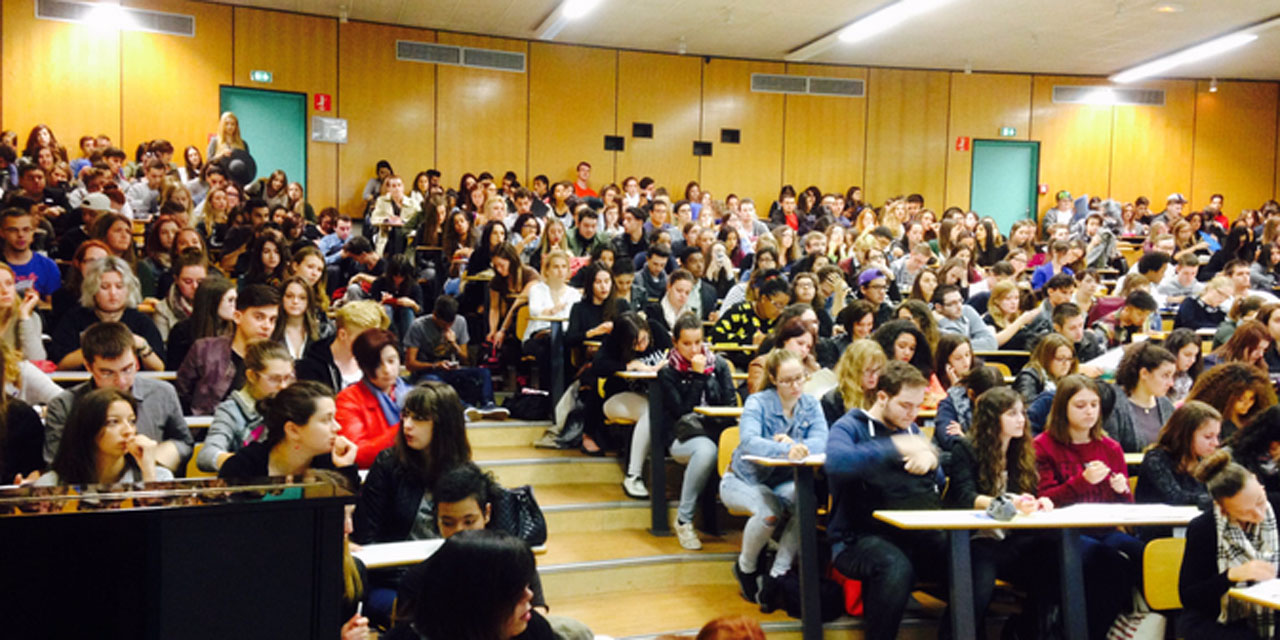
\includegraphics[scale=0.125]{classe.png}
            % }
            \only<1-2>{
              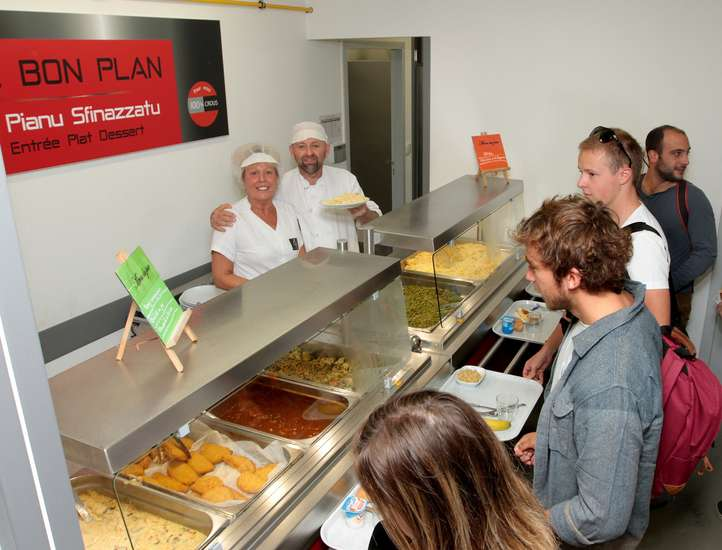
\includegraphics[scale=0.18]{restou.jpg}
            }
            \only<3-4>{
              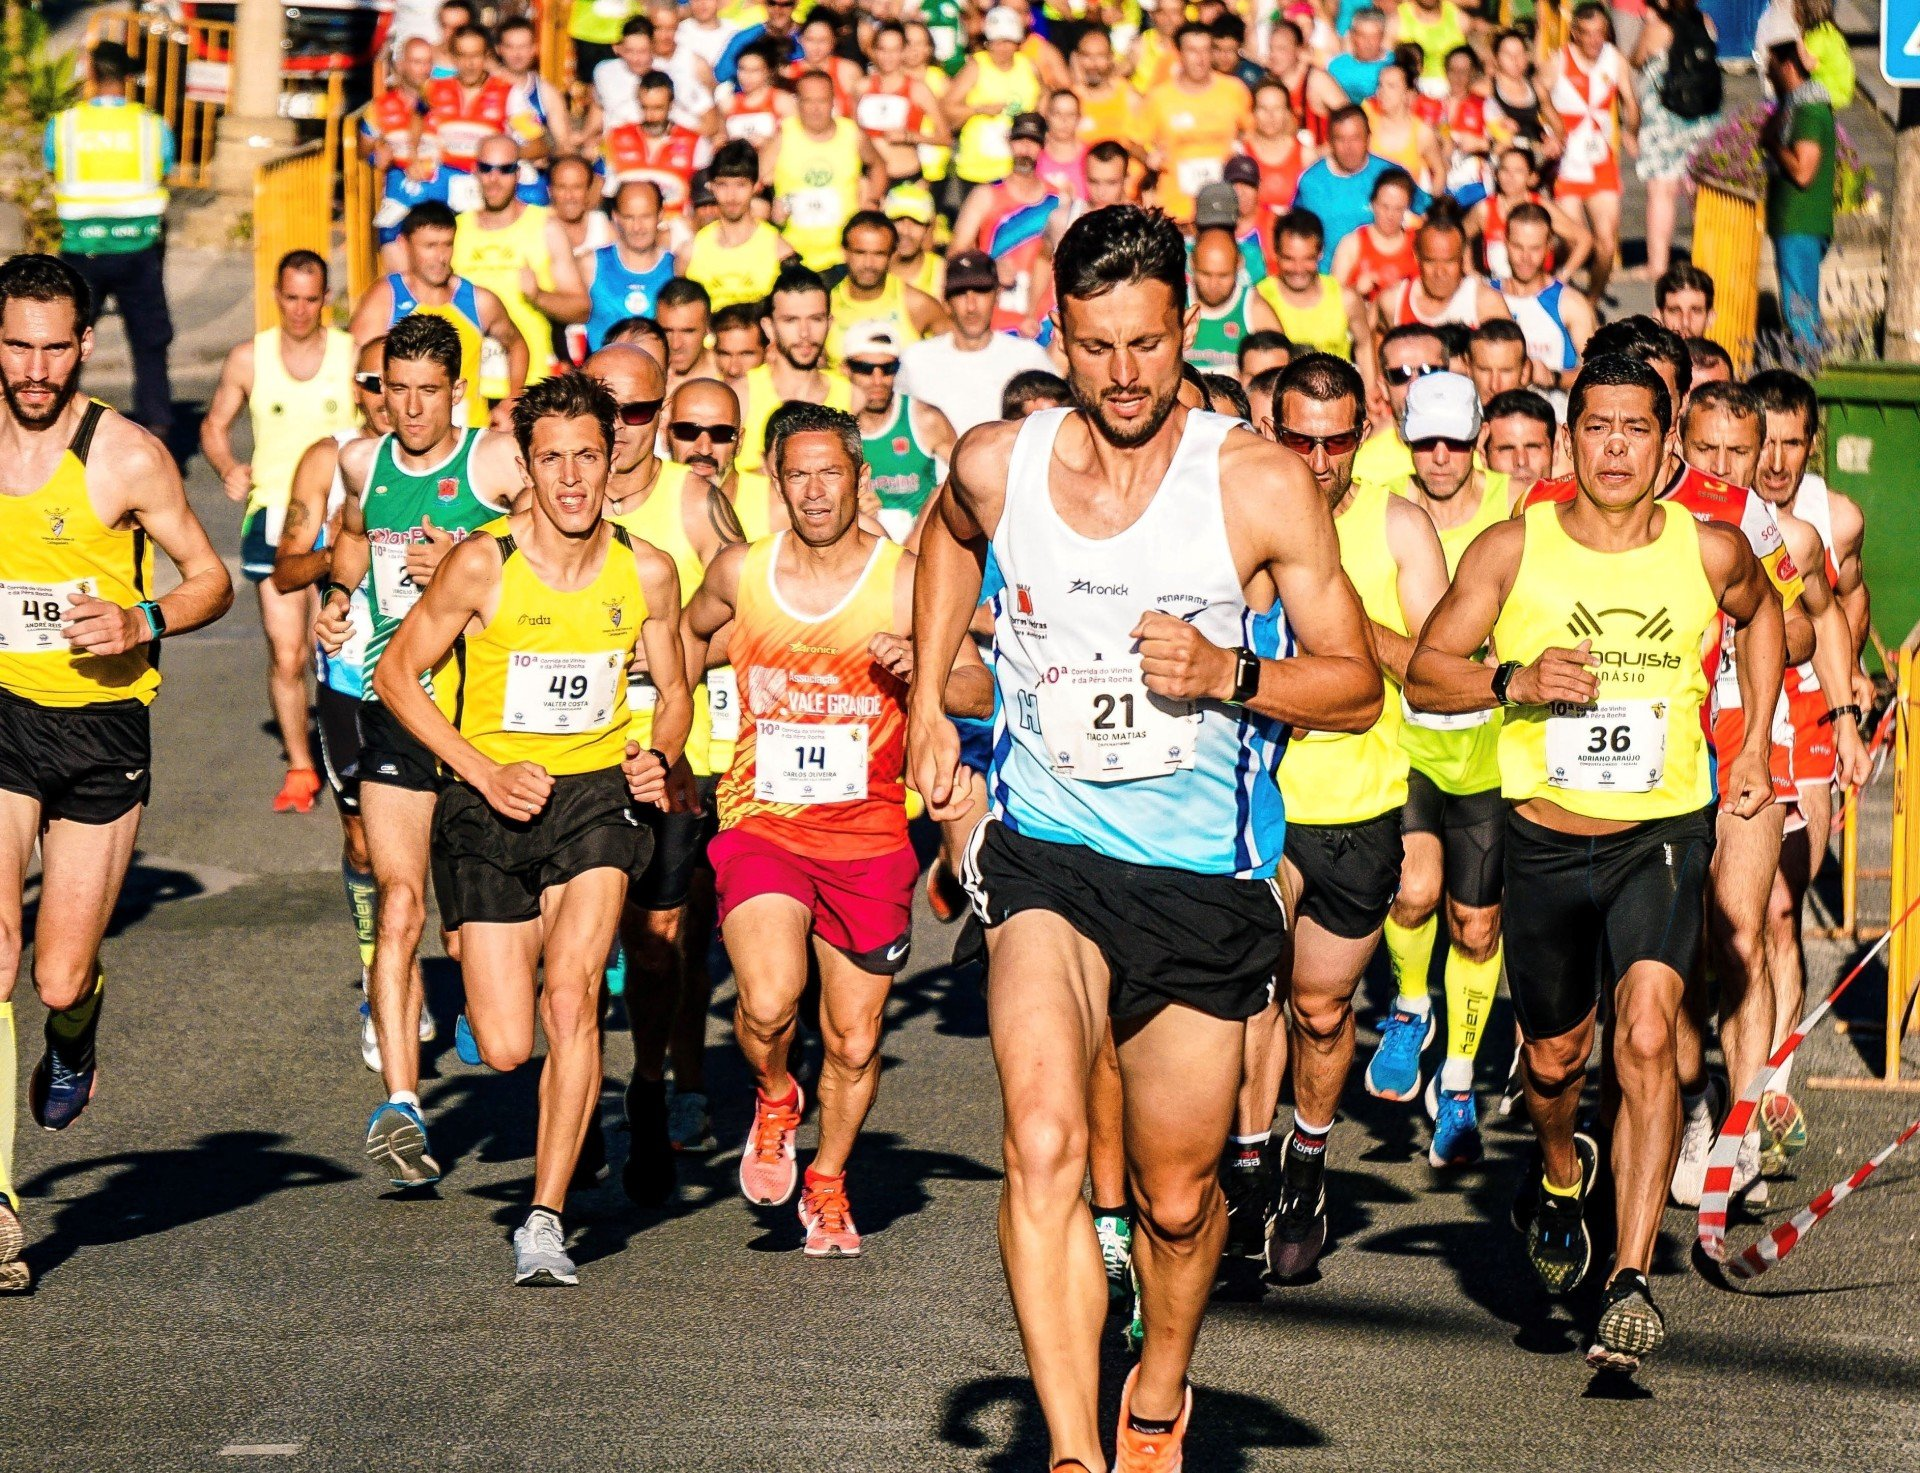
\includegraphics[scale=0.09]{marathon.jpg}
            }
            \only<5-6>{
              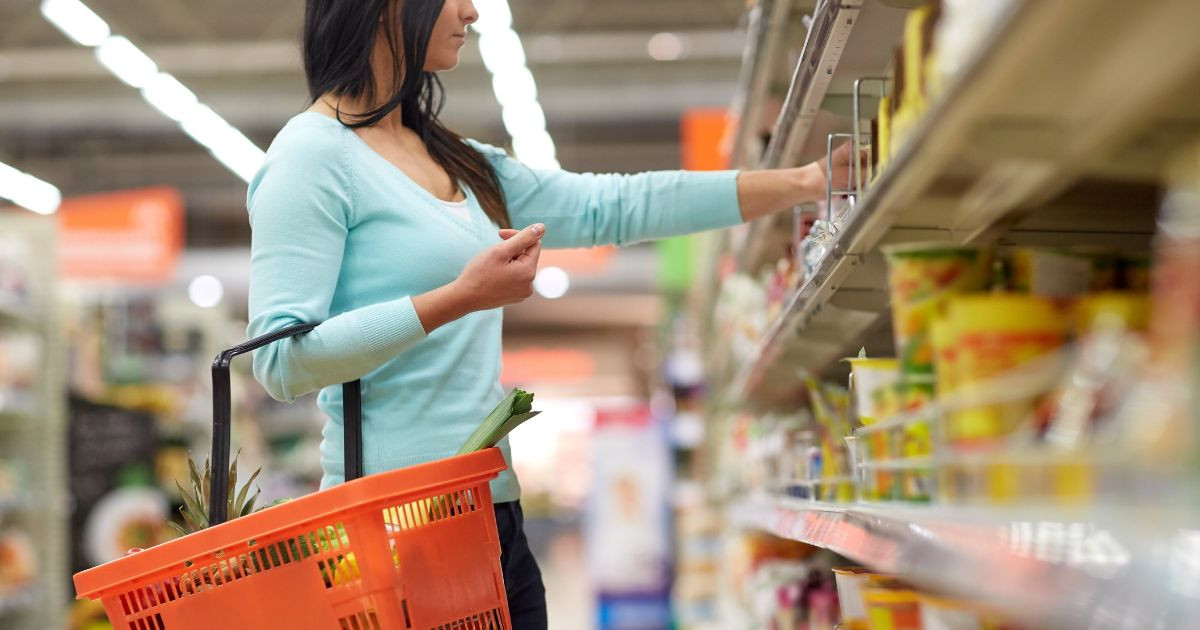
\includegraphics[scale=0.18]{courses.jpg}
            }
            \only<7-8>{
              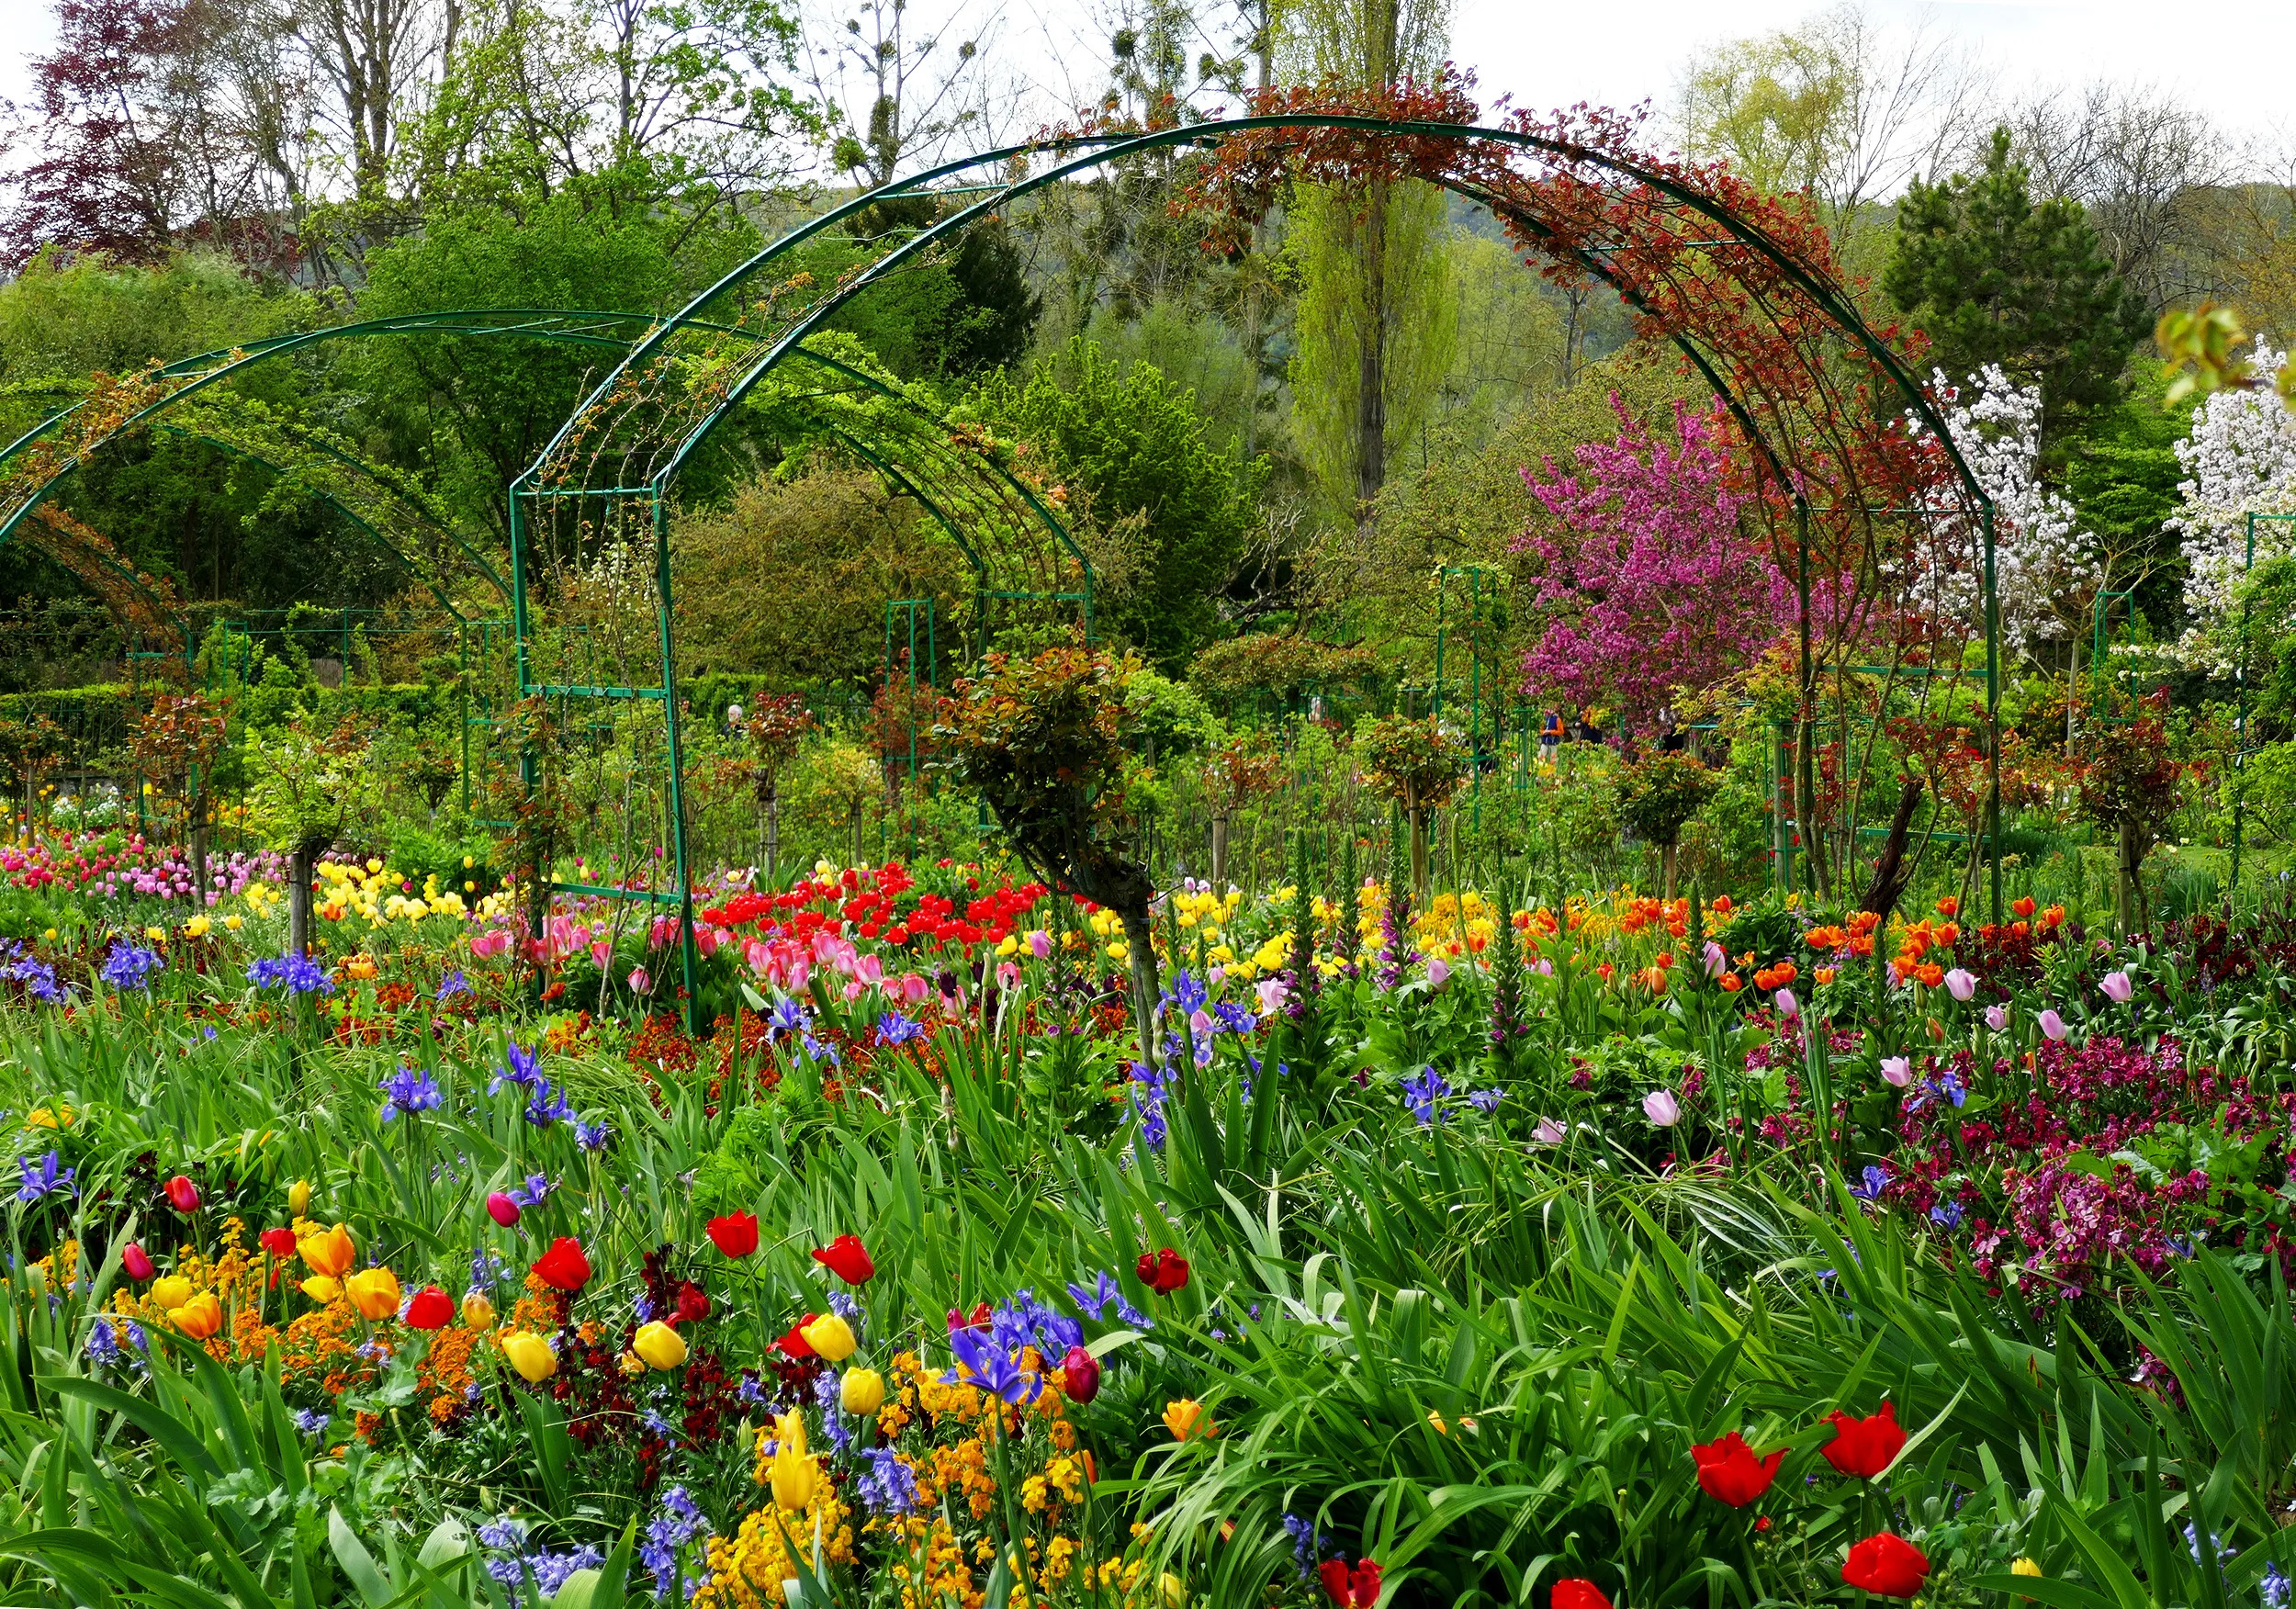
\includegraphics[scale=0.07]{giverny.jpg} \\
              Le jardin de Monet à Giverny
            }
            \only<9-10>{
              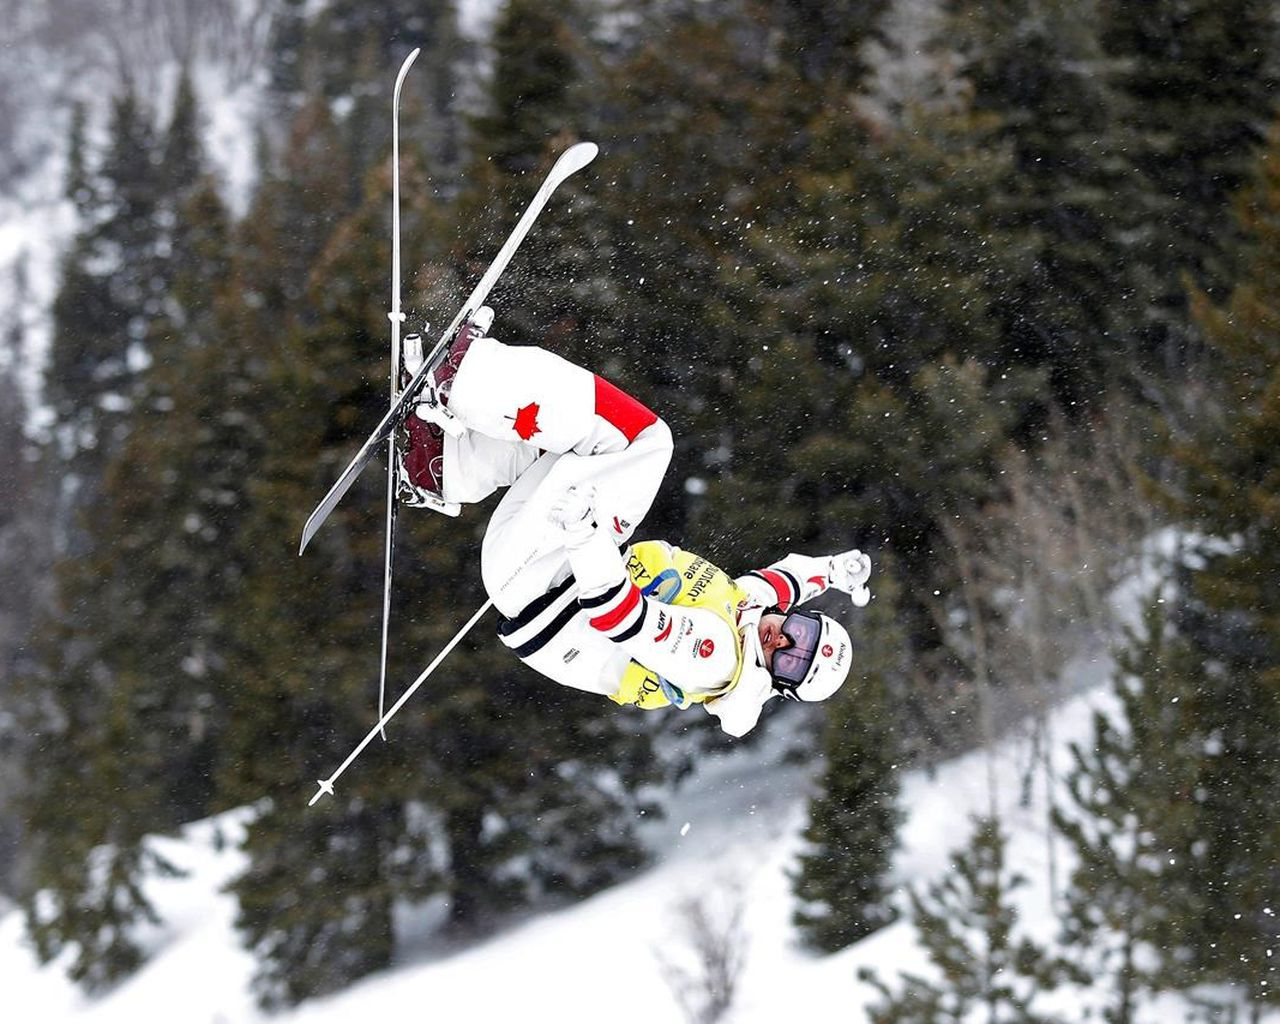
\includegraphics[scale=0.125]{kingsbury.jpg} \\
              Mikaël Kingsbury du Québec
            }
            \only<11-12>{
              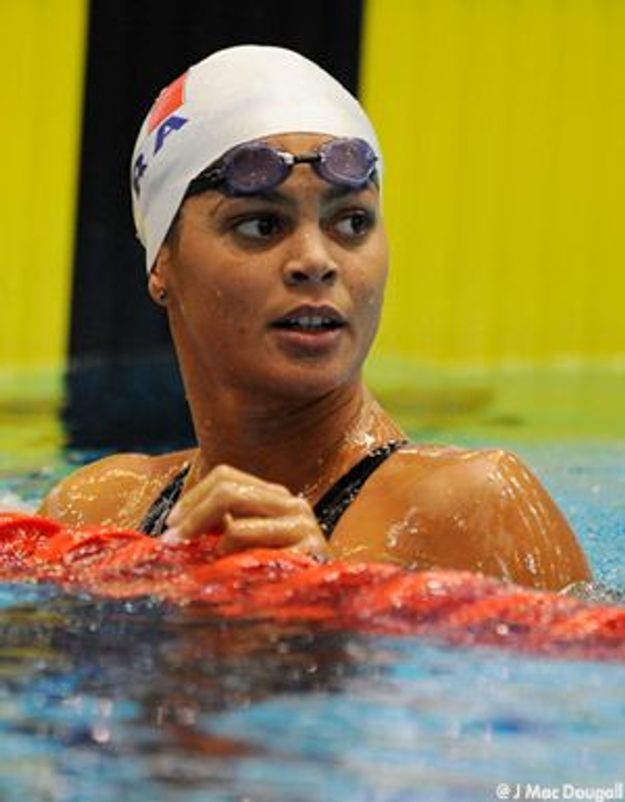
\includegraphics[scale=0.2]{balmy.jpg} \\
              Coralie Balmy de la Martinique
            }
            \only<13-14>{
              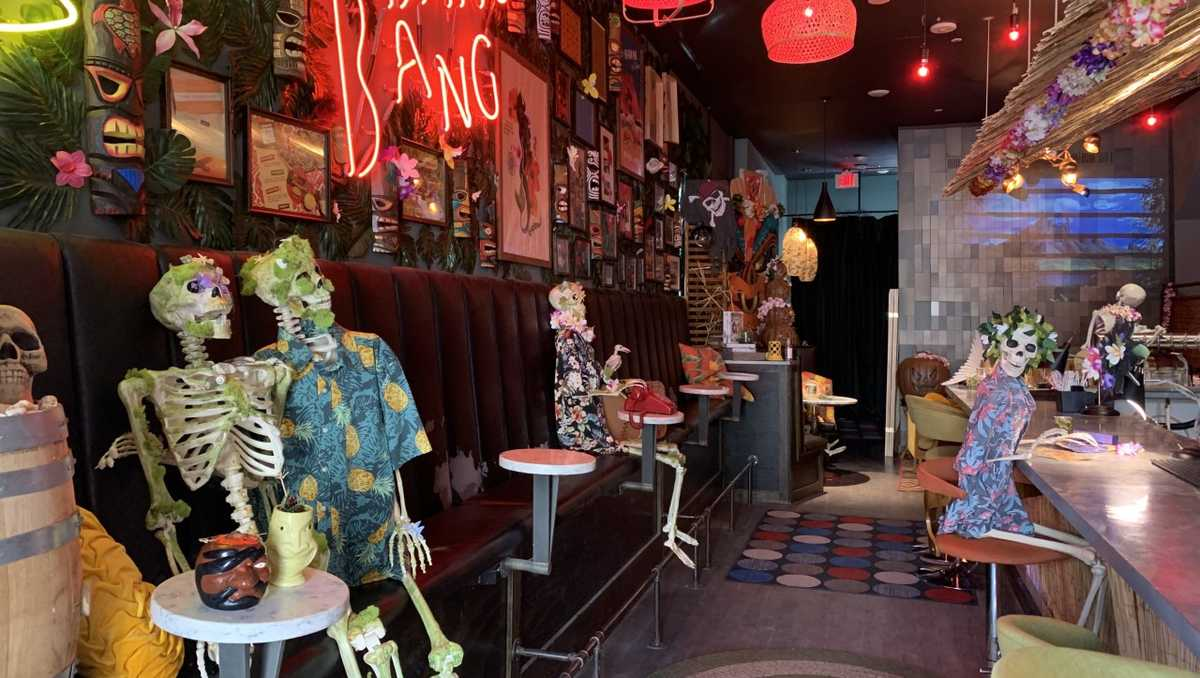
\includegraphics[scale=0.14]{bar_halloween.jpg}
            }
          \end{center}
        \end{minipage}
    \end{columns}
  \end{frame}

  \begin{frame}{Mettez ou jetez?}
    Avec un/e partenaire, décidez si vous allez \textbf{mettre} les articles suivants ou les \textbf{jeter} (dans la poubelle). \\
    \tinygloss{With a partner, decide you will \textbf{put/try on} the following articles or \textbf{throw them out} (in the trash).} \\
    \begin{description}
      \item[\textbf{Modèle:}] \emph{un teeshirt blanc de l'université}
      \item[E1:] Tu mets ce teeshirt.
      \item[] \tinygloss{You put on this T-shirt.}
      \item[] \emph{une robe démodée}
      \item[E2:] Tu dois jeter cette robe.
      \item[] \tinygloss{You must throw out this dress.}
    \end{description}
    \begin{columns}
      \column{0.5\textwidth}
        \begin{enumerate}
          \item des bottes chic
          \item un teeshirt serré
          \item des gants roses, violets et noirs
          \item un manteau trop large
          \item un pantalon trop court
        \end{enumerate}
      \column{0.5\textwidth}
        \begin{enumerate}
          \setcounter{enumi}{5}
          \item une belle écharpe
          \item des baskets à la mode
          \item un blouson démodé
          \item un vieux pull
          \item des mocassins démodés
        \end{enumerate}
    \end{columns}
  \end{frame}

  \begin{frame}{Marier let vêtements}
    Avec un/e partenaire, décide ce qui va bien avec chaque article. \\
    \tinygloss{With a partner, decide what goes well with each article.}
    \begin{description}
      \item[] \textbf{Modèle:} \lexi{avec une robe bleue en soie}
      \item[E1:] Avec une robe bleue en soie, on peut mettre un foulard bleu et vert.
      \item[] \tinygloss{With this blue silk dress, one can put on a blue and green scarf.}
      \item[E2:] Et des chausseurs à talons.
      \item[] \tinygloss{And some high-heeled shoes.}
    \end{description}
    \begin{columns}
      \column{0.45\textwidth}
        \begin{enumerate}
          \item avec une mini-jupe rouge
          \item avec un costume bleu
          \item avec un pantalon bleu
          \item avec une veste noire
        \end{enumerate}
      \column{0.55\textwidth}
        \begin{enumerate}
          \setcounter{enumi}{4}
          \item avec une belle jupe multicolore
          \item avec un tailleur pantalon marron
          \item avec un jean
          \item avec un pantalon noir en cuir
        \end{enumerate}
    \end{columns}
  \end{frame}

  \begin{frame}{}
    \begin{center}
      \Large Questions?
    \end{center}
  \end{frame}
\end{document}
